\chapter{Pioneiras: A história das primeiras mulheres na análise do comportamento no Brasil}\sectionmark{Pioneiras: A história das primeiras mulheres na análise do comportamento no Brasil}
\begin{flushright}
\begin{scriptsize}
Gabriela Jheniffer Teixeira Silva\footnote{Graduanda do curso de Psicologia da Universidade Federal de São Carlos.} \& Ana Arantes\footnote{Pesquisadora de Pós-doutorado do Programa de Pós-graduação em Psicologia (Comportamento e Cognição), docente e pesquisadora associada do Departamento de Psicologia da Universidade Federal de São Carlos.} \footnote{Este capítulo é proveniente da Monografia de Bacharelado da primeira autora, orientada pela segunda autora e apresentada ao Departamento de Psicologia da Universidade Federal de São Carlos (UFSCar) como uma das exigências para finalização do curso de graduação em Psicologia.}
\end{scriptsize}
\vspace{1cm}

\emph{De fato, eu me arriscaria a supor que Anônimo,\\
que escreveu tantos poemas sem assiná-los,\\
foi muitas vezes uma mulher.\\
(Virgínia Wolf, 1928)}
\end{flushright}

Pensar na ciência como um campo (majoritariamente) masculino não é algo recente. Pelo contrário, um dos primeiros estudos a abordar a diferença na produção científica entre homens e mulheres foi realizado por Rossi (1965). Apesar de esse estudo ter sido conduzido há mais de 50 anos, seus resultados infelizmente podem ser facilmente extrapolados para este século. Mulheres tinham menor participação na produção científica em diversas áreas e, de acordo com a autora, isso poderia ser explicado pela falta de incentivo e desencorajamento sistemático, desde a idade escolar, para que mulheres se engajassem em atividades que não as preparassem para seu futuro ideal: ser esposa e mãe (Rossi, 1965). Historicamente, as mulheres foram domesticadas para, independentemente de sua formação, suas maiores conquistas serem um bom casamento e a criação de filhos (ver, por exemplo, Rossi, 1965 e Foucault, 2003). Além disso, existia ainda uma restrição em aceitar mulheres em cursos do ensino superior, apoiada nos estereótipos acima citados (Nosik, 2018).

Apesar das mudanças relacionadas à aceitação e aos direitos conquistados na segunda metade do século XX e às lutas dos movimentos feministas em busca de igualdade entre homens e mulheres, ainda hoje, em pleno século XXI, são palpáveis as diferenças entre gêneros quanto ao acesso à riqueza, direitos e oportunidades (ONU, 2015, \textit{Minimum Set of Gender Indicators}). Para Bourdieu essas mudanças sociais não resolvem a questão da desigualdade, pois:

\begin{quote}
(...) mesmo quando as pressões externas são abolidas e as liberdades formais – direito de voto, direito à educação, acesso a todas as profissões, inclusive políticas – são adquiridas, a autoexclusão e a ‘vocação’ (...) vêm substituir a exclusão expressa (Bourdieu, 1998, p. 52, citado por Moraes, 2012).
\end{quote}

Ou seja, a crença de que homens e mulheres teriam mais chances de alcançar sucesso de acordo com suas supostas características e qualidades inerentes fundamenta e perpetua a disparidade entre gêneros em diversos âmbitos profissionais, incluindo a ciência (Souza \& Fonseca, 2008). Uma rápida análise histórica e cultural demonstra os diversos estigmas e consequentes dificuldades do ser mulher num campo que não fosse o papel tradicional: mãe, esposa e responsável pelas tarefas domésticas. De fato, as diferenças biológicas existem, mas em muitos casos elas se tornam a justificativa e não a causa das diferenças culturais. (Macêdo \& Macedo, 2004; Araújo, 2005; Moraes, 2012; e Da Silva, 2015).

Este movimento de exclusão e impedimento do envolvimento de mulheres na área científica pode ser definido como o silenciamento e a invisibilização feminina que acontecem dentro do contexto social considerado comum. O sujeito (ou grupo) coexiste em dimensões paralelas da realidade instituída, que ressignificam o ser humano constantemente tendo como base as circunstâncias a que está submetido, englobando o trabalho, a política e a sexualidade. Essas variáveis seriam, então, cruciais para a construção não só do sujeito em si, mas da sua representação diante da sociedade (Da Silva, 2015). Como descrito pela autora, silenciamento e invisibilização explicitam os mecanismos pelos quais se marginalizam as minorias sociais:

\begin{quote}
O processo de silenciamento compõe a tríade: ausência de discurso, discurso como monólogo e discurso não considerado. Por sua vez, o processo de invisibilização estabelece a tríade: sujeito inconveniente, sujeito ignorado e o não-sujeito (pp. 113-114)
\end{quote}

O silenciamento das mulheres na área científica ocorre pela ausência de discurso como quando não se criam condições para que mulheres sejam palestrantes em eventos científicos, pela falta de convite por parte dos organizadores ou pela imposição de exigências que impossibilitam que elas apresentem seus trabalhos (como a exigência de que palestras sejam proferidas apenas por Doutores, o que impede que a maioria das mulheres, concentrada nos níveis de graduação e mestrado, tenha oportunidade de palestrar). O discurso como monólogo silencia as mulheres nas ciências quando são impedidas de expor pontos de vista particularmente femininos pelo fato de serem obrigadas a seguir normatizações e procedimentos que limitam o discurso ao ponto de vista dominante e único dos homens, como a norma gramatical de se usar o pronome masculino como padrão, por exemplo. Já o discurso não considerado silencia as mulheres em áreas científicas em que proposições femininas são diminuídas ou consideradas equivocadas pelo simples fato de serem emitidas por mulheres, o que pode ser visto nas críticas infundadas à prática da terapia feminista como antiética, baseadas na noção de que existiria uma “ideologia feminista” que estaria sendo imposta ao cliente por parte da terapeuta.

Em relação à tríade de invisibilização, podemos compreender o sujeito inconveniente como aquele considerado indesejado pela sociedade, um incômodo que deve ser evitado e que é caracterizado, por exemplo, por regras não explícitas do tipo “pós-graduandas mulheres atrasam a defesa de seus projetos porque engravidam durante o curso”, que podem gerar preferência pela seleção de alunos homens por programas de pós-graduação, evitando a seleção de mulheres. O sujeito ignorado é aquele que, apesar de presente, não tem suas contribuições levadas em conta, exemplificado claramente pelo fenômeno do \textit{mansplaining}, em que mulheres, mesmo que com comprovada expertise em seus campos de atuação, são submetidas a situações em que homens explicam a elas os conceitos de suas especialidades de maneira condescendente e simplificada, ignorando que a mulher possa dominar o assunto em questão. E, por fim, o não-sujeito é aquele que sequer é considerado uma pessoa e passa a ser tratado como objeto, como coisa. Muitas vezes as mulheres são aceitas em laboratórios científicos não por suas contribuições intelectuais, mas por sua força de trabalho considerada meticulosa e perfeccionista, como se fossem equipamentos de pesquisa e não pesquisadoras.

Invisibilização e silenciamento podem ser observados também na associação automática que leitoras e leitores fazem ao se deparar com referências em artigos acadêmicos, feitas somente com o sobrenome da pessoa que escreveu o trabalho citado: se presume que autores de trabalhos acadêmicos são necessariamente do gênero masculino, mesmo em áreas predominantemente femininas, como a Psicologia, por exemplo. Outro caso parecido que podemos listar são os inúmeros feitos e pesquisas que foram realizados e/ou tiveram uma importante participação de mulheres cujos nomes são geralmente esquecidos. Não são apenas nomes ignorados, mas também e principalmente são histórias perdidas no tempo. Um dos casos mais emblemáticos é o de Rosalind Franklin. Foi a partir dos dados da pesquisa desta química britânica que foi possível elaborar o modelo de dupla hélice do DNA. Os dois cientistas – homens – que apresentaram tal descoberta para a comunidade científica foram gratificados com um Prêmio Nobel e, somente décadas depois, foi reconhecida a importância da participação de Franklin (Ortiz \& Silva, 2016). Outro caso que representa bem o machismo científico foi o de Nettie Stevens, uma das pioneiras no desenvolvimento de estudos genéticos que foram cruciais para a descoberta de que os determinantes do sexo de um organismo seriam cromossomos e não fatores ambientais. Apesar de um colega de laboratório ter chegado aos mesmos resultados tempos depois de Stevens, a descoberta foi creditada a ele, juntamente com o supervisor do laboratório em que trabalhavam (Lee, 2013).

Um estudo realizado por West, Jacquet, King, Correll e Bergstrom (2013) mostra que aproximadamente 70\% da produção científica mundial até o ano de 2012 era de autoria de homens. Para explicar esta disparidade, existe um conceito cunhado por Rossiter (1993) denominado “Efeito Matilda”, que descreve o sub-reconhecimento de cientistas do gênero feminino nas áreas acadêmicas por meio da invisibilização e apagamento de suas contribuições, como nos casos citados de Franklin e Stevens. As possíveis justificativas para este efeito são o fato das mulheres estarem mais propensas a deixar a academia por fatores pessoais, mais especificamente, devido ao acúmulo de jornadas de trabalho, resultado de uma distribuição ineficiente das responsabilidades domésticas. (Sousa \& Guedes, 2016). Esse desequilíbrio entre o trabalho e a vida pessoal interfere diretamente na produtividade e avanço destas cientistas. (Knobloch-Westerwick, Glynn, \& Huge, 2013). Outro fator apontado é a participação das mulheres em redes de colaboração: enquanto mulheres são mais propensas a colaborar com outros cientistas (independentemente de seu gênero), as redes de colaboração de homens têm como padrão ser composta quase exclusivamente por outros homens. Esses padrões na comunicação acadêmica podem ser cumulativos, levando à impossibilidade das mulheres acadêmicas se desenvolverem em suas carreiras (Knobloch-Westerwick et. al., 2013).

Rossi (1965) aponta possíveis caminhos para que uma sociedade e, consequentemente, uma ciência mais igualitária sejam alcançadas: 1) educar crianças de formas similares, para que papéis familiares e profissionais tenham o mesmo peso independente do gênero de quem os desempenha; e 2) entender que as possíveis dificuldades que uma mulher possa encontrar ao desempenhar uma profissão que exija mais dedicação não estão ligadas a sua (falta de) capacidade e sim ao acúmulo de papéis (esposa, mãe, profissional) e, a partir disso, compreender que isso é um problema social e histórico, e não individual – atuando para que tal informação seja difundida e esta questão seja trabalhada em conjunto com a sociedade. Rossi (1965) aponta também que o aumento no número de mulheres cientistas seria uma das ferramentas para provocar as modificações coletivas necessárias para se alcançar a igualdade.

\section{Psicologia: Uma profissão feminina, mas uma ciência masculina}

Diante desse quadro de silenciamento das mulheres e de invisibilização da presença feminina no campo científico, não surpreende que, mesmo em áreas majoritariamente femininas, possamos verificar como as contribuições das mulheres são menos reconhecidas do que aquelas feitas por homens. Um caso emblemático a ser exemplificado é o das ciências psicológicas, cuja área (tanto acadêmica e científica, quanto aplicada) é formada por 90\% de profissionais mulheres, segundo levantamento do DIEESE (2016) sobre os dados da PNAD (Pesquisa Nacional por Amostra de Domicílio) realizada pelo IBGE (Instituto Brasileiro de Geografia e Estatística) em 2014.

A graduação em Psicologia, desde a sua fundação, foi composta por uma maioria esmagadora de mulheres (Rosemberg, 1984). Existem diversas variáveis que contribuem para a explicação desse fenômeno, como o possível reflexo dos modelos sexuais tradicionais (o que reservaria à mulher o papel de sentimental e “expressiva”), e a segregação ocupacional, que delega às mulheres profissões ligadas diretamente ao cuidado doméstico e com outras pessoas (Rosemberg, 1984). Essa presença expressiva das mulheres nas graduações em Psicologia não se traduz necessariamente em participação efetiva na construção da Psicologia como profissão e como corpo de conhecimento. Dados recentes mostram que, no Brasil, há uma desproporção na presença de mulheres em relação à de homens conforme nos dirigimos a níveis mais altos da carreira. Por exemplo, as mulheres representam 90\% do total de profissionais de psicologia formadas e formados no país, mas a porcentagem de professoras mulheres cai drasticamente para 56,6\% dos professores de ensino superior em Psicologia (DIEESE, 2016). Pensando na produção científica, mulheres são maioria desde a graduação até o nível do Pós-doutorado, mas coordenam apenas cerca de 40\% de grandes projetos de pesquisa (Costa, 2006), o que pode até soar relevante, no entanto a autora aponta que, ainda que não exista um preconceito explícito, as estruturas sociais (família, religião, economia, direito, etc.) e a cultura agem “de forma a garantir a hegemonia masculina nos postos mais elevados das ciências.” (p.458). Embora esses dados sejam sobre a participação feminina nas ciências em geral, e de não termos dados específicos sobre a participação feminina na Psicologia em particular, é de se esperar, considerando a literatura sobre invisibilização e silenciamento, que na nossa área essa tendência se repita.
\vfill

\section{Por que estudar a história da Análise do Comportamento no Brasil?}

Mesmo que não se tenha dados, específicos ou gerais, e estudos sobre a participação e contribuição das mulheres na ciência psicológica no Brasil, pensamos que um estudo sobre as desigualdades entre gêneros, particularmente dentro da Análise do Comportamento (AC), pode servir como caso exemplar. A chegada da AC coincide com o desenvolvimento institucionalizado do curso de Psicologia no país, o que provavelmente é uma das razões para que tenha se tornado uma disciplina de currículo mínimo da graduação (Miranda \& Cirino, 2010) e colocado o Brasil entre os países em que a pesquisa científica na área seja uma das mais expressivas. 

Poucos anos após a vinda da AC para o Brasil, nos anos 1960, ocorreu o golpe militar. Tal fato impossibilitou um pleno desenvolvimento desta ciência naquele momento (Ferreira, 1985; Matos \& Carvalho, 1998). Ferreira (1985) afirma que cientistas brasileiros encontravam sérias limitações para o desenvolvimento da Psicologia como ciência por causa de um sistema de comunicação pobre entre os profissionais e por dificuldades econômicas do país que resultavam em cortes constantes de fundos para pesquisa e programas de graduação e pós-graduação descontinuados, chegando ao ponto de as próprias universidades não terem dinheiro suficiente para comprar livros e manter a assinatura de diversos periódicos. De acordo com Matos e Carvalho (1998), uma das principais dificuldades enfrentadas foi a falta de equipamentos e bibliografias necessários aqui no Brasil, o que também refletia diretamente na aprendizagem dos alunos. Durante a ditadura militar, os analistas do comportamento se viram obrigados, por conta das restrições pessoais, políticas e econômicas impostas, a voltar-se para a aplicação clínica e ensino. Houve diversos cancelamentos de viagens para o exterior, assim como dificuldades na importação de materiais e revogação de convites para professores de outros países virem ao Brasil por conta das restrições xenófobas impostas pelos militares (Todorov, 2004). 

Mesmo com este percalço, nem tudo foi perdido. Os trabalhos desenvolvidos na Universidade de Brasília (UnB) resultaram em publicações nacionais e internacionais significativas (Matos \& Carvalho, 1998). Além disso, por conta da dispersão dos profissionais pelo país, com o passar dos anos, muitos cursos de graduação em Psicologia tiveram em suas primeiras matrizes a influência direta do trabalho de Carolina Bori (Todorov \& Hanna, 2010).

A constante produção de pesquisas em AC (básicas, aplicadas e conceituais) desde a década de 1960, a realização sistemática de diversos eventos científicos e o número crescente de periódicos e livros especializados são aspectos que fundamentam a importância de estudos históricos sobre a área no nosso país. Como destaca Cruz (2006), embora existam poucos exemplos de pesquisas históricas sobre a AC no Brasil, tais pesquisas podem ser instigantes e reveladoras e, principalmente, auxiliar no delineamento da produção de conhecimento na área. Apesar da pouca produção relativa a pesquisas históricas, nos últimos anos houve um aumento substancial de pesquisas voltadas para a análise histórico-conceitual, o que indica a consolidação da AC na comunidade científica, uma vez que a área se desenvolveu o suficiente para buscar, em sua história, aspectos relevantes que favorecem a identificação de fatores que estão constantemente afetando a constituição da AC e do Behaviorismo no Brasil (Cruz, 2006). 

\section{Presença e participação feminina na Análise do Comportamento brasileira}

No decorrer da história da AC no Brasil, diversas mulheres tiveram papéis importantes, algumas vezes até cruciais para o estabelecimento da área no país, mas pouco se tem registrado sobre suas contribuições. Um bom exemplo disso é o fato quase desconhecido de que o primeiro convite para que o Professor Keller\footnote{O Professor Fred S. Keller, em 1961, veio ao Brasil lecionar durante um ano como professor visitante na Universidade de São Paulo. No decorrer da disciplina de Psicologia Experimental, o Prof. Keller não só apresentava o conteúdo programático da AC, como administrava exercícios práticos em laboratório. Estas aulas foram a primeira semente da Análise Experimental do Comportamento no nosso país (Matos \& Carvalho, 1998).} viesse para o Brasil partiu de uma aluna do curso de Psicologia da Universidade de São Paulo, Mirtes Rodrigues do Prado (Couto, 2012). Uma das poucas mulheres com reconhecimento mais amplo dentro do campo da ciência psicológica foi a Professora Doutora Carolina Martuscelli Bori que, nas palavras de Matos e Carvalho (1998), conquistou este posto por “principalmente ao longo de várias gestões como parte da Diretoria da SBPC”, ter rompido “os tabus políticos mais resistentes deste país: uma mulher à frente dos cientistas brasileiros” (p.5).

Como já discutido, a invisibilização do trabalho feminino é histórica e não exclusiva do campo da Psicologia ou da AC – é uma opressão estrutural (Velho \& León 2012). Resgatar e trazer à tona o trabalho dessas mulheres é uma forma não só de resgatar ângulos não explorados da história da AC brasileira, como também de ir contra o movimento de apagamento dessa parte importante da história das mulheres que fazem e contribuem significativamente para a ciência. Por isso, neste estudo, pretendemos apresentar como a produção e a carreira acadêmico-científica dessas mulheres vêm sendo retratada pela área e investigar o papel que a presença feminina teve na constituição e consolidação da AC no Brasil. Para esse objetivo, realizamos um levantamento bibliográfico em nove bases de dados de periódicos científicos e em quatro periódicos nacionais da área de AC (como mostrado na Tabela 1), sem restrição de data, utilizando as seguintes combinações de buscadores: “início da Análise do Comportamento”, “história”, “Análise do Comportamento”, “Brasil”, “mulheres”, “behaviorismo”, e “pesquisa histórica”, bem como suas respectivas traduções para o inglês.

% Please add the following required packages to your document preamble:
% \usepackage{booktabs}
\begin{table}[]
\caption{Lista de bases de dados e periódicos da área de AC usados no levantamento bibliográfico.}
\begin{adjustbox}{max width=1\textwidth}
\begin{tabular}{@{}l@{}}
\toprule
\multicolumn{1}{c}{\textbf{Bases de dados}}                                     \\ \midrule
Biblioteca Nacional de Medicina dos Estados Unidos (PubMed)                     \\
Biblioteca Virtual em Saúde - Psicologia Brasil (Bvs-Psi)                       \\
Centro Latino-Americano e do Caribe de Informação em Ciências da	Saúde (Bireme) \\
\textit{Education Resources Information Center  (Eric)}                                  \\
Periódicos Eletrônicos em Psicologia (PEPsic)                                   \\
\textit{American Psychological Association (PsycInfo})                                   \\
\textit{Scientific	Electronic Library Online (Scielo) }                                  \\
\textit{SciVerse Scopus (Scopus)}                                                        \\
\textit{Web	of Science}                                                               \\ \midrule
\multicolumn{1}{c}{\textbf{Periódicos nacionais de Análise do Comportamento}}   \\ \midrule
\textit{\textit{Acta Comportamentalia*}}                                                 \\
Revista Brasileira de Terapia Comportamental e Cognitiva (RBTCC)                \\
Revista Perspectivas em Análise do Comportamento                                \\
Revista Brasileira de Análise do Comportamento (REBAC)                          \\ \bottomrule
\end{tabular}
\end{adjustbox}
\caption*{*Apesar de ser um periódico internacional, os artigos selecionados neste periódico foram publicados em português, portanto optamos por incluí-lo na categoria de publicação nacional.}
\end{table}

Inicialmente, foram selecionados todos os artigos que continham um ou mais dos buscadores citados e aqueles que mostrassem uma ou mais palavras-chave semelhante aos buscadores utilizados. A partir do título, resumo e, se necessário, a leitura completa do artigo, foram selecionados aqueles trabalhos que abordavam, por meio de estudos de caso ou históricos, os 20 primeiros anos da AC no Brasil e aqueles que continham informações históricas ou documentação sobre este período. Foram encontrados 2730 artigos e, destes, 16 foram selecionados seguindo os critérios descritos.

A Figura 1.1 mostra a distribuição de artigos publicados por ano sobre a temática. Mesmo sem a existência de limitação de período temporal nas buscas, somente dois artigos foram publicados antes do ano 2000 e a maioria (nove dos 16 artigos) se concentra no período pós-2010. Esta informação corrobora o trabalho de Cruz (2006), comprovando a existência de uma lacuna a ser preenchida nesse âmbito, uma vez que existem poucas pesquisas históricas acerca da AC no país.

\begin{figure}[h]
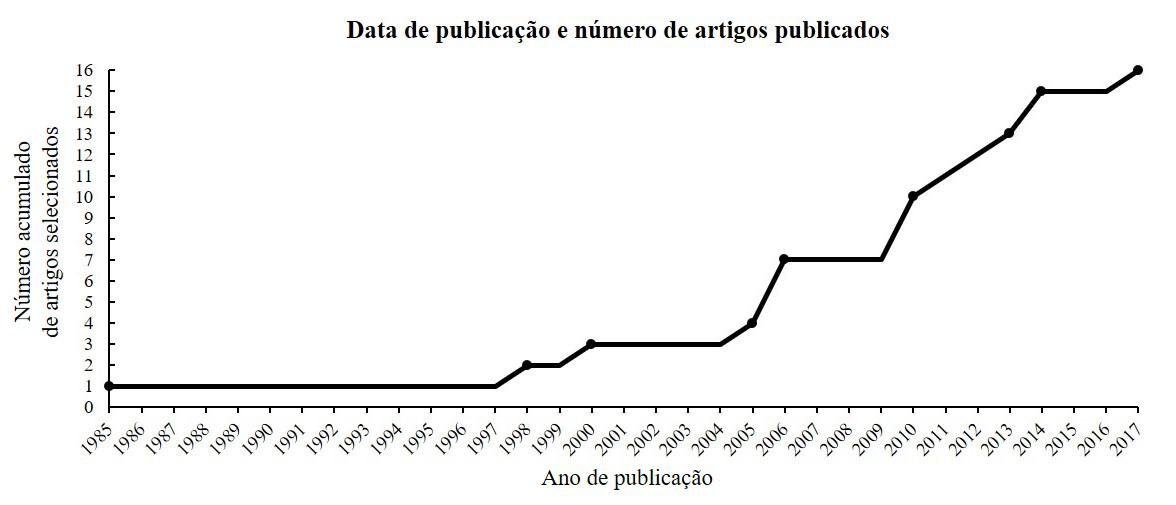
\includegraphics[width=1\textwidth]{1/figura1}
\captionof{figure}{Distribuição do número de artigos encontrados de acordo com as datas de publicação dos mesmos. A curva acumulada mostra o crescimento acelerado de publicações sobre história da AC a partir de 2010.}
\end{figure}

Ao se buscar um resgate histórico da construção de uma ciência, como no caso da AC, é crucial considerar que a relação entre o comportamento do cientista, a comunidade científica e o contexto cultural em que cientista e comunidade se inserem são aspectos indissociáveis. A complexidade e a amplitude dessas variáveis nos impossibilitam contar toda a história e estamos limitadas e limitados, de forma que qualquer tentativa de concretizar tal tarefa resulta em esboços da história. (Cruz, 2006). Tais esboços, entretanto, não perdem seu valor porque tornam possível identificar ao menos algumas das variáveis presentes na cultura daquele momento que se relacionam com o comportamento não só de uma cientista ou um cientista, mas de toda uma comunidade científica, de acordo com o contexto cultural e histórico (Cruz, 2006). Este capítulo é um exemplo de como podemos utilizar essas relações para recontar a história, estando nós mesmas inseridas num contexto diferente e analisar, com base nas informações atuais, como se deu a construção da AC para compreender como e por que se deu o apagamento sistemático de inúmeras histórias e contribuições de mulheres ao longo do desenvolvimento da área.

\begin{figure}
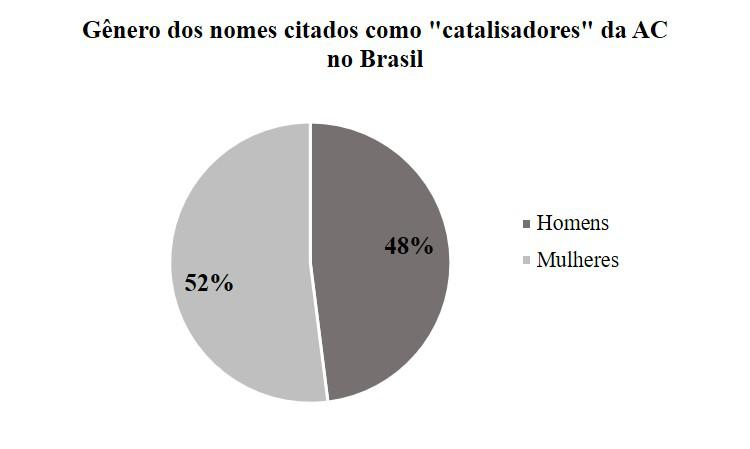
\includegraphics[width=1\textwidth]{1/figura2}
\captionof{figure}{Distribuição por gênero dos nomes da área de AC, citados nos artigos selecionados para o estudo, considerados “catalisadores” da AC no Brasil entre 1960 e 1985.}
\end{figure}

Os artigos selecionados na busca relatavam acontecimentos ocorridos entre 1960 e 1985, configurando os primeiros 25 anos da AC no país, e citavam um total de 55 nomes da pesquisa e da academia na área de AC e Behaviorismo Radical. Dentre esses, 29 eram mulheres, configurando 52\% do total, como podemos observar na Figura 2. A participação feminina no início da AC brasileira parece seguir a tendência expressa na Psicologia como um todo, demonstrada anteriormente, em que a participação das mulheres cai de 89\% de estudantes na graduação em Psicologia (Rosemberg, 1984) para uma participação de 56,6\% nos quadros docentes (DIEESE, 2016), e continua diminuindo para 52\% das pesquisadoras consideradas importantes para “catalisação” da AC. Pode parecer uma comparação entre desiguais, dado que se compara a porcentagem total de alunas de graduação nos cursos de Psicologia com a porcentagem de pesquisadoras cujos papéis dentro da área de AC são considerados fundantes. Porém, é de se pensar como os homens passam de 11\% dos estudantes de graduação em Psicologia daquela época (entre 1960 e 1980) para mais da metade dos grandes pesquisadores de uma ciência, enquanto a maioria das mulheres não ultrapassa os níveis da graduação e pós-graduação. Dado o contexto histórico do início da AC no Brasil, podemos buscar compreender esses dados como resultado dos papéis de gênero fortemente arraigados que desestimulavam então, e ainda desestimulam hoje, um maior envolvimento feminino profissional e acadêmico.

Mesmo com representação ligeiramente diminuída, relativamente à representação dos homens (29 mulheres para 26 homens citados), os números apresentados são importantes, pois salientam que apesar de todo o contexto histórico envolvido, mulheres estiveram e foram presentes ativamente na formação de analistas do comportamento e na disseminação de laboratórios de Análise Experimental do Comportamento pelo país. Mostram também como a percepção do papel das mulheres na área é subestimada pelas próprias cientistas e pelos próprios cientistas, já que um levantamento informal entre colegas analistas do comportamento tende a mostrar que, além das Professoras Carolina Bori, Maria Amélia Matos e algumas outras, a maioria das pesquisadoras e dos pesquisadores de AC não tem informações sobre essa participação fundamental das mulheres na área.

Dentre os 16 artigos selecionados para este estudo, 62\% deles são de autoria estritamente masculina. Esse dado é muito interessante se levarmos em consideração a discussão acerca do “Efeito Matilda” e como o gênero influencia nas escolhas de coautores: a maioria esmagadora dos artigos é escrita somente por homens e, em sua maioria, somente com outros homens como parceiros. Esse dado, aliado às informações já citadas da acerca da proporção de mulheres na Psicologia, nos mostra que esse efeito não acontece por falta de profissionais femininas nas áreas científicas, mas porque homens sistematicamente excluem as mulheres do fazer científico. Pode-se inferir, portanto, que é mais um exemplo prático do “Efeito Matilda”.

A representação das mulheres na AC vem sendo analisada há tempos no âmbito internacional. O trabalho de Poling et al. (1983) foi pioneiro desta área ao avaliar a contribuição das mulheres na produção científica da área no que diz respeito à autoria dos artigos publicados e na participação de mulheres nos conselhos editoriais dos principais periódicos internacionais. Esse estudo mostrou tendências crescentes na representação das mulheres como analistas do comportamento, ainda que essa participação não seja representativa do total de mulheres na área, em relação ao número relativo de homens. A pesquisa de Nosik (2018) mostra um aumento considerável da participação feminina na AC em diversas faixas etárias, o que demonstra que o aumento de cientistas mulheres é uma das ferramentas necessárias para promover mudanças de contingências necessárias para se alcançar a equidade, mesmo que os avanços sejam feitos aos poucos (Rossi, 1965).

Ao longo da leitura dos artigos selecionados para este estudo, percebemos que a participação feminina na formação da AC como área científica no Brasil se deu, principalmente, em três categorias de atuação distintas, ainda que sobrepostas em alguns casos: 1. a importância dessas profissionais no ensino da AC durante os anos iniciais da Psicologia no Brasil; 2. suas contribuições para o conhecimento analítico-comportamental nas áreas de pesquisa básica e aplicada; e 3. seu papel na difusão da AC como ciência e das tecnologias advindas desta. Desse modo, foi possível compreender de maneira mais acurada como se deram suas contribuições ao longo da formação da AC no país. A Tabela 1.2 mostra a distribuição das mulheres mencionadas nos artigos selecionados entre categorias formuladas. A atribuição das analistas do comportamento às categorias se deu seguindo os seguintes critérios:

\begin{enumerate}[1. ]
\item Contribuições Para o Ensino: quando, nos artigos selecionados, foram citadas informações acerca da carreira docente como Universidade, período de docência, disciplinas ministradas e afins.

\item Contribuições Científicas (Pesquisa): quando foram descritos o desenvolvimento ou estabelecimento de linhas de pesquisa e de laboratórios e/ou participação e orientação de alunos em laboratórios de pesquisa.

\item Contribuições Para a Difusão da AC: quando foram encontradas informações sobre a elaboração de livros para públicos diversos, participação na consolidação de políticas públicas, fundação ou participação em cursos de outras áreas (pedagogia, biologia, enfermagem, etc.), clínicas e institutos.
\end{enumerate}

% Please add the following required packages to your document preamble:
% \usepackage{booktabs}
% \usepackage{multirow}
\begin{table}[]
\caption{Categorização da participação feminina na formação da AC, segundo os artigos selecionados para o estudo.}
\begin{adjustbox}{max width=1\textwidth}
\begin{tabular}{@{}ccc@{}}
\toprule
\textbf{Categoria}                                                         & \textbf{Referência}                                           & \textbf{Analistas do comportamento citadas} \\ \midrule
\multicolumn{1}{c|}{\multirow{8}{*}{Ensino}}                               & \multicolumn{1}{c|}{\multirow{2}{*}{Barbosa et al., 2017}}    & Ana Lúcia Ulian                             \\
\multicolumn{1}{c|}{}                                                      & \multicolumn{1}{c|}{}                                         & Sandra Eli Bachiega                         \\ \cmidrule(l){2-3} 
\multicolumn{1}{c|}{}                                                      & \multicolumn{1}{c|}{\multirow{2}{*}{Miranda \& Cirino, 2010}} & Carolina Bori                               \\
\multicolumn{1}{c|}{}                                                      & \multicolumn{1}{c|}{}                                         & Maria Amélia Matos                          \\ \cmidrule(l){2-3} 
\multicolumn{1}{c|}{}                                                      & \multicolumn{1}{c|}{\multirow{4}{*}{Todorov \& Hanna, 2010}}  & Margarida Windholz                          \\
\multicolumn{1}{c|}{}                                                      & \multicolumn{1}{c|}{}                                         & Dora Fix Ventura                            \\
\multicolumn{1}{c|}{}                                                      & \multicolumn{1}{c|}{}                                         & Maria Inês Rocha e Silva                    \\
\multicolumn{1}{c|}{}                                                      & \multicolumn{1}{c|}{}                                         & Vera Konigsberger                           \\ \midrule
\multicolumn{1}{c|}{\multirow{10}{*}{Contribuição científica (Pesquisa)}}  & \multicolumn{1}{c|}{\multirow{6}{*}{Miranda \& Cirino, 2010}} & Maria Amélia Matos                          \\
\multicolumn{1}{c|}{}                                                      & \multicolumn{1}{c|}{}                                         & Dora Fix                                    \\
\multicolumn{1}{c|}{}                                                      & \multicolumn{1}{c|}{}                                         & Rachel Kerbauy                              \\
\multicolumn{1}{c|}{}                                                      & \multicolumn{1}{c|}{}                                         & Maria José Vasconsellos                     \\
\multicolumn{1}{c|}{}                                                      & \multicolumn{1}{c|}{}                                         & Adélia Teixeira                             \\
\multicolumn{1}{c|}{}                                                      & \multicolumn{1}{c|}{}                                         & Sonia dos Santos Castanheira                \\ \cmidrule(l){2-3} 
\multicolumn{1}{c|}{}                                                      & \multicolumn{1}{c|}{\multirow{3}{*}{Todorov \& Hanna, 2010}}  & Elenice Ferrari                             \\
\multicolumn{1}{c|}{}                                                      & \multicolumn{1}{c|}{}                                         & Deisy das Graças de Souza                   \\
\multicolumn{1}{c|}{}                                                      & \multicolumn{1}{c|}{}                                         & Herma Drachenberg                           \\ \cmidrule(l){2-3} 
\multicolumn{1}{c|}{}                                                      & \multicolumn{1}{c|}{Fidalgo, 2014}                            & Carolina Bori                               \\ \midrule
\multicolumn{1}{c|}{\multirow{16}{*}{Difusão da Análise do Comportamento}} & \multicolumn{1}{c|}{\multirow{2}{*}{Miranda \& Cirino, 2010}} & Carolina Bori                               \\
\multicolumn{1}{c|}{}                                                      & \multicolumn{1}{c|}{}                                         & Maria Amélia Matos                          \\ \cmidrule(l){2-3} 
\multicolumn{1}{c|}{}                                                      & \multicolumn{1}{c|}{Todorov \& Hanna, 2010}                   & Maria Helena Leite Hunziker                 \\ \cmidrule(l){2-3} 
\multicolumn{1}{c|}{}                                                      & \multicolumn{1}{c|}{Polanco, 2014}                            & Ione Scarpelli Pereira                      \\ \cmidrule(l){2-3} 
\multicolumn{1}{c|}{}                                                      & \multicolumn{1}{c|}{\multirow{12}{*}{Barbosa et al., 2017}}   & Mercedes Cunha de Carvalho                  \\
\multicolumn{1}{c|}{}                                                      & \multicolumn{1}{c|}{}                                         & Marilena Ristum                             \\
\multicolumn{1}{c|}{}                                                      & \multicolumn{1}{c|}{}                                         & Márcia Bonagamba                            \\
\multicolumn{1}{c|}{}                                                      & \multicolumn{1}{c|}{}                                         & Vera Otero                                  \\
\multicolumn{1}{c|}{}                                                      & \multicolumn{1}{c|}{}                                         & Marlene Gonzales                            \\
\multicolumn{1}{c|}{}                                                      & \multicolumn{1}{c|}{}                                         & Anamélia Araújo de Carvalho                 \\
\multicolumn{1}{c|}{}                                                      & \multicolumn{1}{c|}{}                                         & Ana Cecília Sousa Bittencourt Bastos        \\
\multicolumn{1}{c|}{}                                                      & \multicolumn{1}{c|}{}                                         & Ana Helena Galvão                           \\
\multicolumn{1}{c|}{}                                                      & \multicolumn{1}{c|}{}                                         & Márcia Miriam Gomes                         \\
\multicolumn{1}{c|}{}                                                      & \multicolumn{1}{c|}{}                                         & Liana Sodré                                 \\
\multicolumn{1}{c|}{}                                                      & \multicolumn{1}{c|}{}                                         & Zorilda Goes                                \\
\multicolumn{1}{c|}{}                                                      & \multicolumn{1}{c|}{}                                         & Profa. Luzidéia*                           
\end{tabular}
\end{adjustbox}
\caption*{*Não há informações sobre o nome completo dessa analista do comportamento.}
\end{table}

De um total de 29 mulheres citadas como “catalisadoras” e pioneiras da consolidação da AC no Brasil, quatro dos 16 artigos selecionados apresentam a maioria das mulheres (16 citadas) na categoria de Difusão da Análise do Comportamento, novamente seguindo a tendência, verificada tanto em outras áreas da Psicologia quanto dentro da AC, da presença feminina mais expressiva nas áreas aplicadas (ou seja, na prestação de serviços psicológicos) do que nas áreas científicas. Nas categorias de Contribuição Científica (Pesquisa) e de Ensino foram alocadas 10 e oito analistas do comportamento, respectivamente. Nota-se, também, que as Professoras Carolina Bori e Maria Amélia Matos aparecem nas três categorias, atestando sua importância para a AC brasileira. A Professora Dora Fix Ventura tem seu papel categorizado, também, tanto em Contribuição Científica (Pesquisa) como em Ensino. Em contraste com esse reconhecimento da área a essas pesquisadoras e professoras, temos o nome da Professora Luzidéia, citada no artigo de Barbosa, Costa, Ulian e Lima (2017), sobre a qual não encontramos maiores informações, nem mesmo sobre seu nome completo. O fato de essa professora ser somente citada em um estudo sobre a AC no Nordeste, região historicamente negligenciada nas políticas educacionais e científicas do país, não nos foge à atenção.

Para uma melhor visualização e entendimento do desenvolvimento da AC no Brasil através das contribuições das mulheres da área, foi elaborada uma linha do tempo com as informações coletadas nos artigos selecionados, mostrada na Tabela 1.3. Podemos ver, nessa cronologia, a expressiva participação das mulheres desde o lançamento das bases experimentais da AC no Brasil, com a fundação de laboratórios experimentais e intercâmbio com pesquisadores internacionais já estabelecidos, passando pelo ensino de disciplinas de Análise Experimental do Comportamento e outras disciplinas de Psicologia sob a ótica analítico-comportamental, até o início da clínica comportamental, estabelecendo a área aplicada e a prestação de serviços em Análise do Comportamento Aplicada.
\vfill
\pagebreak

\scriptsize
% Please add the following required packages to your document preamble:
% \usepackage{booktabs}
% \usepackage{longtable}
% Note: It may be necessary to compile the document several times to get a multi-page table to line up properly
\begin{longtable}{@{}ccc@{}}
\caption{Linha do tempo das participações e contribuições das mulheres analistas do comportamento nos primeiros 20 anos da AC no Brasil, conforme descrito nos artigos selecionados para este estudo.}\\
\toprule
\textbf{Período} & \textbf{Participação das analistas do comportamento}                                                                                                                                                                                                                                                                                                                                                                                                                                                                                                                                                                                                    & \textbf{Referências}                                                                         \\* \midrule
\endhead
%
1960-1970        & \begin{tabular}[c]{@{}c@{}}Deisy das Graças de Souza, então bolsista\\ de iniciação científica, Elenice Ferrari e outros estudantes\\ desenvolvem pesquisas sobre controle aversivo,\\ reconhecidas por sua qualidade e originalidade\\ e publicadas em revistas internacionais.\end{tabular}                                                                                                                                                                                                                                                                                                                                                           & Todorov \& Hanna, 2010                                                                       \\* \midrule
1961             & \begin{tabular}[c]{@{}c@{}}Maria Amélia Matos, Dora Fix Ventura,\\ Margarida Windholz, Vera Konigsberger e\\ Maria Inês Rocha e Silva são as primeiras alunas\\ do curso oferecido por Keller durante sua\\ primeira vinda ao Brasil.\end{tabular}                                                                                                                                                                                                                                                                                                                                                                                                      & Todorov \& Hanna, 2010                                                                       \\* \midrule
1961-1962        & \begin{tabular}[c]{@{}c@{}}Maria Amélia Matos e Carolina Bori trabalham\\ como assistentes do professor Keller.\\ Foram responsáveis pelo primeiro\\ laboratório de AC no Brasil.\end{tabular}                                                                                                                                                                                                                                                                                                                                                                                                                                                          & Cirino, 2012                                                                                 \\* \midrule
1962             & \begin{tabular}[c]{@{}c@{}}Bori se torna uma das primeiras professoras de\\ Psicologia do curso de Pedagogia da Faculdade de Filosofia, \\ Ciências e Letras da cidade de Rio Claro, interior de SP. \\ \\ Herma Drachenberg, sob supervisão de Carolina Bori,\\ esenvolve em conjunto com outro cientista\\ um protótipo do \textit{Personalized System of Instruction} \\ (PSI, da sigla em inglês para Sistema Personalizado de Ensino)\end{tabular}                                                                                                                                                                                                          & Todorov \& Hanna, 2010                                                                       \\* \midrule
1963-1964        & \begin{tabular}[c]{@{}c@{}}Carolina Bori lidera a formação do Departamento\\ de Psicologia da Universidade de Brasília (UnB).\end{tabular}                                                                                                                                                                                                                                                                                                                                                                                                                                                                                                              & Cirino, 2012                                                                                 \\* \midrule
1965             & \begin{tabular}[c]{@{}c@{}}Maria Helena Leite Hunziker e outro cientista\\ fundam o primeiro centro voltado para\\ formação de AC da cidade de Campinas-SP.\end{tabular}                                                                                                                                                                                                                                                                                                                                                                                                                                                                                & Hanna \& Todorov, 2010                                                                       \\* \midrule
1968             & \begin{tabular}[c]{@{}c@{}}Criação do curso de Psicologia na\\ Universidade Federal da Bahia.\\ Profa. Mercedes Cunha de Carvalho é uma das\\ principais colaboradoras, participando da elaboração\\ da grade curricular.\end{tabular}                                                                                                                                                                                                                                                                                                                                                                                                                  & Barbosa et al., 2017                                                                         \\* \midrule
1969             & \begin{tabular}[c]{@{}c@{}}Carolina Bori ministra um curso que versa sobre\\ Psicologia Social Experimental, considerado\\ marco para o início da AC na Universidade\\ Federal de Minas Gerais (UFMG). \\ \\ Ione Scarpelli Pereira, então professora da UFMG,\end{tabular}                                                                                                                                                                                                                                                                                                                                                                             & \begin{tabular}[c]{@{}c@{}}Miranda \& Cirino, 2010\\ \\ \\ Polanco, 2014\end{tabular}        \\* \midrule
1969-1971        & \begin{tabular}[c]{@{}c@{}}Bori ministra aulas no programa de pós-graduação\\  em Psicologia Experimental da USP.\\ \\ Alguns dos principais trabalhos em AC no início\\ da década de 1970 são orientados por Bori. \\ \\ Maria Amélia Matos é responsável por montar\\ o laboratório de comportamento operante,\\ trazendo material dos EUA para a UFMG. \\ \\ Dora Fix coordena o Laboratório\\ de Psicologia Sensorial da UFMG.\\ Carolina Bori e Maria Amélia Matos recebem\\ professores de outras universidades interessados em AC\\ (intercâmbio entre UFMG e USP-São Paulo)\end{tabular}                                                        & \begin{tabular}[c]{@{}c@{}}Miranda \& Cirino, 2010\\ \\ \\ Nale, 1998\end{tabular}           \\* \midrule
1969-1979        & \begin{tabular}[c]{@{}c@{}}Todas as pesquisas sobre comportamento\\ verbal produzidas neste período\\ (totalizando seis estudos) são orientadas\\ por Carolina Bori – enquanto professora da USP.\end{tabular}                                                                                                                                                                                                                                                                                                                                                                                                                                          & Fidalgo, 2014                                                                                \\* \midrule
1970             & \begin{tabular}[c]{@{}c@{}}Rachel Kerbauy escreve o manual “Análise Experimental\\ do Comportamento: exercícios de laboratório”,\\ utilizado amplamente no desenvolvimento do laboratório\\ de AC na UFMG. Seus métodos foram minuciosamente\\ seguidos por discentes e docentes. Maria José Vasconcellos e\\ Sonia Castanheira atuam neste laboratório\\ \\ (Uma curiosidade: o primeiro laboratório de pombos da UFMG\\ foi montado dentro de um dos banheiros do departamento.)\end{tabular}                                                                                                                                                         & \begin{tabular}[c]{@{}c@{}}Miranda \& Cirino, 2010\\ \\ \\ Polanco, 2014\end{tabular}        \\* \midrule
1970-1971        & \begin{tabular}[c]{@{}c@{}}Sonia Santos Castanheira, graduada em Psicologia\\ pela UFMG, que se tornara professora da mesma\\ universidade nos anos 60, inicia pesquisas em AC\\ envolvendo pombos no laboratório didático.\end{tabular}                                                                                                                                                                                                                                                                                                                                                                                                                & Cirino, 2012                                                                                 \\* \midrule
1971             & \begin{tabular}[c]{@{}c@{}}Redação do Regulamento do Laboratório de Psicologia\\ da UFMG, documento assinado por\\ Sonia dos Santos Castanheira.\\ \\ Carolina Bori auxilia na instalação do\\ laboratório de Psicologia Experimental da\\ Universidade Federal do Maranhão (UFMA).\\ Na época foram contratadas duas psicólogas\\ recém-formadas para ministrar aulas:\\ Marilena Ristum e Márcia Bonagamba.\end{tabular}                                                                                                                                                                                                                              & \begin{tabular}[c]{@{}c@{}}Miranda \& Cirino, 2010\\ \\ \\ Barbosa et al., 2017\end{tabular} \\* \midrule
1971-1972        & \begin{tabular}[c]{@{}c@{}}As docentes Maria José Vasconsellos e Maria Amélia Matos\\ são responsáveis pelo I Encontro de Psicologia Experimental\\ na Faculdade de Filosofia e Ciências Humanas da UFMG.\end{tabular}                                                                                                                                                                                                                                                                                                                                                                                                                                  & Miranda \& Cirino, 2010                                                                      \\* \midrule
1972             & \begin{tabular}[c]{@{}c@{}}Vera Otero e Marlene Gonzales substituem\\ Ristum e Bonagamba em seu trabalho na UFMA.\end{tabular}                                                                                                                                                                                                                                                                                                                                                                                                                                                                                                                          & Barbosa et al., 2017                                                                         \\* \midrule
1973             & \begin{tabular}[c]{@{}c@{}}Anamélia Araújo de Carvalho assume a coordenação\\ do Laboratório e o ensino de Psicologia Experimental da \\ Universidade Federal da Bahia (UFBA),\\ junto com algumas egressas como\\ Ana Cecília Sousa Bittencourt Bastos, Ana Helena Galvão,\\ Márcia Miriam Gomes, dentre outras.\\ Este grupo é o primeiro a exercer profissionalmente a\\ terapia comportamental em Salvador-BA.\end{tabular}                                                                                                                                                                                                                         & Barbosa et al., 2017                                                                         \\* \midrule
1974             & \begin{tabular}[c]{@{}c@{}}Adélia Teixeira é orientanda de\\ Doutorado de Bori na USP-SP.\end{tabular}                                                                                                                                                                                                                                                                                                                                                                                                                                                                                                                                                  & Miranda \& Cirino, 2010                                                                      \\* \midrule
1979             & \begin{tabular}[c]{@{}c@{}}Ana Lúcia Ulian, formada pela\\ Universidade de Londrina(UEL) juntamente com\\ Liana Sodré e Zorilda Goes integraram o grupo de\\ ensino da disciplina de Psicologia Experimental da UFBA.\end{tabular}                                                                                                                                                                                                                                                                                                                                                                                                                      & Barbosa et al., 2017                                                                         \\* \midrule
1984             & \begin{tabular}[c]{@{}c@{}}Ana Lúcia Ulian assume a coordenação do\\ Laboratório e as disciplinas de\\ \\ Psicologia Experimental 1 e 2 da UFBA\\ (trabalhos que reveza com outro professor).\\ Estas disciplinas propunham um programa que\\ se utilizava de artigos com conteúdo clínico e\\ metodologia experimental.\\ \\ Posteriormente faz parte do quadro de supervisores\\ do Estágio em Clínica da mesma universidade.\\ É fundado o segundo curso de Psicologia na\\ Universidade de Fortaleza (UNIFOR).\\ \\ \\ As disciplinas de AC são ministradas pela\\ Profa. Luzidéia, ex-aluna da\\ Universidade Federal do Ceará (UFC).\end{tabular} & Barbosa et al., 2017                                                                         \\* \midrule
1985             & \begin{tabular}[c]{@{}c@{}}A Profa. Sandra Eli Bachiega é contratada\\ pela UFC e se torna responsável por supervisões\\ na área clínica utilizando terapia comportamental.\end{tabular}                                                                                                                                                                                                                                                                                                                                                                                                                                                                & Barbosa et al., 2017                                                                         \\* \bottomrule
\end{longtable}
\normalsize
\vfill
\pagebreak

\section{Considerações Finais}
A invisibilização e o silenciamento das mulheres no contexto científico têm sido mostrados em diversos estudos das áreas de Sociologia, Antropologia e História, desde o impedimento inicial da participação feminina nas universidades, até o completo apagamento das cientistas responsáveis por descobertas críticas para a evolução científica em seus campos. Na Psicologia de modo geral, e na AC em particular, esse cenário não é diferente, porém a AC tem progressivamente reparado essa desigualdade histórica reconhecendo aos poucos o papel das mulheres pioneiras da área na fundação da ciência e da prestação de serviços em AC no país, muito por iniciativa das próprias pesquisadoras, como este estudo atesta. 

Para uma melhor compreensão das variáveis históricas e sociais implicadas nas práticas culturais de silenciamento e invisibilização das mulheres na sociedade e na ciência é preciso que tenhamos informações mais precisas sobre a presença e a participação feminina, com dados demográficos específicos sobre o número de mulheres nas associações da área, sua participação nos congressos, nas publicações e nos vários campos de aplicação da AC. McSweeney, Donahoe e Swindell (2000) sugerem a aplicação e acompanhamento de estatísticas formais sobre a participação de mulheres e minorias na AC como uma das estratégias para buscar a equidade da produção e do acesso à academia. Dessa forma, teremos um quadro mais preciso da situação de desigualdade entre os gêneros dentro da área, primeiro passo para a proposição de intervenções para modificar os sistemas de opressão de gênero. E, assim como Nosik (2018), encorajamos as futuras pesquisadoras e os futuros pesquisadores a continuar investigando as variáveis ambientais e práticas culturais de desigualdade de gênero e seus impactos, em prol de uma ciência analítico-comportamental mais igualitária.

Por fim, uma observação deve ser feita a respeito do conceito de mulher utilizado neste estudo: partimos do princípio da distinção de categorias de gênero (feminino e masculino) socialmente construídas, de acordo com teóricas feministas como Rubin (1975) e Lerner (1986), e analistas do comportamento feministas como Ruiz (2003)\footnote{Para maiores discussões sobre o conceito de gênero e as considerações analítico-comportamentais feitas a partir dele, ver o capítulo 02 neste livro.}. Entretanto, é importante levar em consideração que a categoria mulher não é única e sim múltipla (Esmeraldo, 2006). Variáveis como raça, orientação sexual, identidade de gênero e classe social das analistas do comportamento pioneiras citadas neste estudo não foram levadas em consideração por falta destas informações em documentos históricos e nos artigos encontrados. Sabe-se, no entanto, que o perfil da população com nível universitário nas décadas de 1960 a 1980, no Brasil, era de homens brancos, heterossexuais e cisgêneros (ao menos publicamente), originários das classes sociais mais altas (Ristoff, 2014). Tendo em vista este contexto histórico-cultural, pode-se inferir que a maioria - para não dizer a totalidade - das mulheres citadas aqui se enquadra nos mesmos padrões de raça, orientação sexual e identidade de gênero públicas, além de compartilharem da mesma classe social. Tais interseccionalidades são frequentemente negligenciadas, portanto é necessária a realização de pesquisas que foquem em tais recortes para que possamos vislumbrar os seus impactos na construção da ciência. Nomes, histórias e contribuições foram e continuam sendo apagadas de forma recorrente – e o caso das mulheres é o mais evidente.

\chapter*{Referências Bibliográficas}\sectionmark{Referências Bibliográficas}
\hangindent=25pt
\hangafter=1
\noindent Araújo, M. F. (2005). Diferença e igualdade nas relações de gênero: Revisitando o debate. \textit{Psicologia Clínica}, 17(2), 41-52.

\hangindent=25pt
\hangafter=1
\noindent Barbosa, J. I. C., Costa, N., Ulian, A. L. A. O, \& Lima, L. S. (2017). Memórias da Análise do Comportamento no Nordeste: Bahia, Ceará e Maranhão. \textit{Revista Brasileira de Terapia Comportamental e Cognitiva}, 19, 61-70.

\hangindent=25pt
\hangafter=1
\noindent Camargo, W. X., \& Kessler, C. S. (2017). Além do masculino/feminino: Gênero, sexualidade, tecnologia e performance no esporte sob perspectiva crítica. \textit{Horizontes Antropológicos}, 47, 191-225.

\hangindent=25pt
\hangafter=1
\noindent Costa, M. C. (2006). Ainda somos poucas: Exclusão e invisibilidade na ciência. \textit{Cadernos Pagu,} 27, 455-459.
 
\hangindent=25pt
\hangafter=1
\noindent Couto, A. (2012). História da Análise do Comportamento no Brasil. \textit{Revista Online Comporte-se: Psicologia e Análise do Comportamento}.  Retirado de: http://www.comportese.com/2012/02/historia-da-analise-do-comportamento-no-brasil/

\hangindent=25pt
\hangafter=1
\noindent Cruz, R. N. (2006). História e Historiografia da Ciência: considerações para pesquisa histórica em análise do comportamento. \textit{Revista Brasileira de Terapia Comportamental e Cognitiva}, 8(2), 161-178. 

\hangindent=25pt
\hangafter=1
\noindent Departamento Intersindical de Estatísticas e Estudos Socioeconômicos. (2016). Levantamento de informações sobre a inserção dos psicólogos no mercado de trabalho brasileiro. Retirado de: \url{http://bit.ly/dieese2016}

\hangindent=25pt
\hangafter=1
\noindent Esmeraldo, G. G. S. L. (2006). O feminismo no plural: Para pensar a diversidade constitutiva das mulheres.\textit{ Revista Estudos Feministas,} 14(3), 829-831.

\hangindent=25pt
\hangafter=1
\noindent Ferreira, M. C. R. (1985). The study of behavioural development in Brazil: Contemporary research, teaching, and practice. \textit{International Journal of Behavioral Development}, 8, 139-151.

\hangindent=25pt
\hangafter=1
\noindent Ferreira, M. C. (2004). Sexismo hostil e benevolente: Inter-relações e diferenças de gênero. \textit{Temas em Psicologia,} 12(2), 119-126.

\hangindent=25pt
\hangafter=1
\noindent Foucault, M. (2003). História da Sexualidade, Volume 1: A vontade de saber. Rio de Janeiro: Graal. (Trabalho original publicado em 1988).

\hangindent=25pt
\hangafter=1
\noindent Knobloch-Westerwick, S., Glynn, C. J., \& Huge, M. (2013). The Matilda effect in science communication: An experiment on gender bias in publication quality perceptions and collaboration interest. \textit{Science Communication,} 35(5), 603-625.

\hangindent=25pt
\hangafter=1
\noindent Lee, J. J. (2013). Six women scientists who were snubbed due to sexism. \textit{National Geographic}. Retirado de: \url{http://bit.ly/leejj2013}

\hangindent=25pt
\hangafter=1
\noindent Lerner, G. (1986). The Creation of Patriarchy. New York: Oxford University Press.

\hangindent=25pt
\hangafter=1
\noindent Macêdo, G. S., \& Macedo, K. B. (2004). As relações de gênero no contexto organizacional: O discurso de homens e mulheres. \textit{Revista Psicologia Organizações e Trabalho}, 4(1), 61-90. 

\hangindent=25pt
\hangafter=1
\noindent Matos, M. A., \& Carvalho, A. M. A. (1998). Carolina Martuscelli Bori: Uma cientista brasileira. \textit{Psicologia: Reflexão e Crítica}, 11(2), 411-420. 
 
\hangindent=25pt
\hangafter=1
\noindent McSweeney, F. K., Donahoe, P., \& Swindell, S. (2000). Women in applied behavior analysis. \textit{The Behavior Analyst}, 23(2), 267-277.

\hangindent=25pt
\hangafter=1
\noindent Miranda, R. L., \& Cirino, S. D. (2010). Os primeiros anos dos laboratórios de análise do comportamento no Brasil. \textit{Psychologia Latina}, 1(1), 79-87.

\hangindent=25pt
\hangafter=1
\noindent Moraes, E. (2012). Ser mulher na atualidade: A representação discursiva da identidade feminina em quadros humorísticos de Maitena. Em I. Tasso \& P. Navarro, (Orgs.), \textit{Produção de identidades e processos de subjetivação em práticas discursivas}, (pp. 259-285). Maringá: Eduem.

\hangindent=25pt
\hangafter=1
\noindent Nosik, M. R., Luke, M. M., \& Carr, J. E. (2018). Representation of women in Behavior Analysis: An empirical analysis. \textit{Behavior Analysis: Research and Practice}, 1(2), 1-9.

\hangindent=25pt
\hangafter=1
\noindent Organização das Nações Unidas. (2015). Minimum Set of Gender Indicators. Disponível em https://genderstats.un.org

\hangindent=25pt
\hangafter=1
\noindent Ortiz, E., \& Silva, M.R. (2016). O uso de abordagens da História da Ciência no ensino de biologia: Uma proposta para trabalhar a participação da cientista Rosalind Franklin na construção do modelo da dupla hélice do DNA. \textit{Investigações em Ensino de Ciências}, 21(1), 106-123. 

\hangindent=25pt
\hangafter=1
\noindent Poling, A., Grossett, D., Fulton, B., Roy, S., Beechler, S., \& Wittkopp, C. J. (1983). Participation by women in behavior analysis.\textit{ The Behavior Analyst,} 6, 145-152.

\hangindent=25pt
\hangafter=1
\noindent Ristoff, D. (2014). O novo perfil do campus brasileiro: Uma análise do perfil socioeconômico do estudante de graduação. \textit{Avaliação: Revista da Avaliação da Educação Superior} (Campinas), 19(3), 723-747.

\hangindent=25pt
\hangafter=1
\noindent Rosemberg, F. (1984). Afinal, por que somos tantas psicólogas? \textit{Psicologia: Ciência e Profissão}, 4(1), 6-12. 

\hangindent=25pt
\hangafter=1
\noindent Rossi, A. (2012). Women in science: Why so few? \textit{Science}, 148(3674), 1196-1202.

\hangindent=25pt
\hangafter=1
\noindent Rossiter, M. W. (1993). The Matthew Matilda effect in science. \textit{Social Studies of Science}, 23(2), 325-341. 

\hangindent=25pt
\hangafter=1
\noindent Rubin, G. (1975). The traffic in women. Em: R. Reiter, (Org.), \textit{Towards an Antropology of Women}, (pp. 160-207). New York: Monthly Review Press. 

\hangindent=25pt
\hangafter=1
\noindent Ruiz, M. R. (2003). Inconspicuous sources of behavioral control: The case of gendered practices. \textit{The Behavior Analyst Today}, 4, 12–16. 

\hangindent=25pt
\hangafter=1
\noindent Da Silva, W.A. (2015). Foucault e indigenciação: As formas de silenciamento e invisibilização dos sujeitos. \textit{Problemata: Revista Internacional de Filosofia}, 6(3), 111-128. 

\hangindent=25pt
\hangafter=1
\noindent Sousa, L. P., \& Guedes, D. R. (2016). A desigual divisão sexual do trabalho: Um olhar sobre a última década. \textit{Estudos Avançados,} 30(87), 123-139. 

\hangindent=25pt
\hangafter=1
\noindent Souza, M. R. F., \& Fonseca, M. C. F. R. (2008). Mulheres, homens e matemática: Uma leitura a partir dos dados do Indicador Nacional de Alfabetismo Funcional. Educação e Pesquisa, 34(3), 511-526. 

\hangindent=25pt
\hangafter=1
\noindent Todorov, J. C., \& Hanna, E. S. (2010). Análise do Comportamento no Brasil. \textit{Psicologia: Teoria e Pesquisa}, 26(SpE), 143-154.

\hangindent=25pt
\hangafter=1
\noindent Todorov, J. C. (2004). Da aplysia à constituição: Evolução de conceitos na análise do comportamento. \textit{Psicologia: Reflexão e Crítica}, 17(2), 151-156.

\hangindent=25pt
\hangafter=1
\noindent Velho, L., \& León, E. (2012). A construção social da produção científica por mulheres. \textit{Cadernos Pagu}, 10, 309-344. 

\hangindent=25pt
\hangafter=1
\noindent Woolf, V. (1985). Um teto todo seu. Rio de Janeiro: Nova Fronteira. (Trabalho original publicado em 1928.)

\hangindent=25pt
\hangafter=1
\noindent West, J. D., Jacquet, J., King, M. M., Correll, S. J., \& Bergstrom, C. T. (2013). \textit{The role of gender in scholarly authorship}. PloS ONE, 8(7), e66212.